\chapter*{付録}
\label{chap:appendix}
\fancyhf{}
\rhead{\thepage}
\lhead{付録:各講座のネットワーク図}
\cfoot{\thepage}

\begin{figure}[!htb]
\begin{center}
	\hspace*{-10pt}\makebox[1.2\textwidth][c]{
		\minipage{0.52\textwidth}
			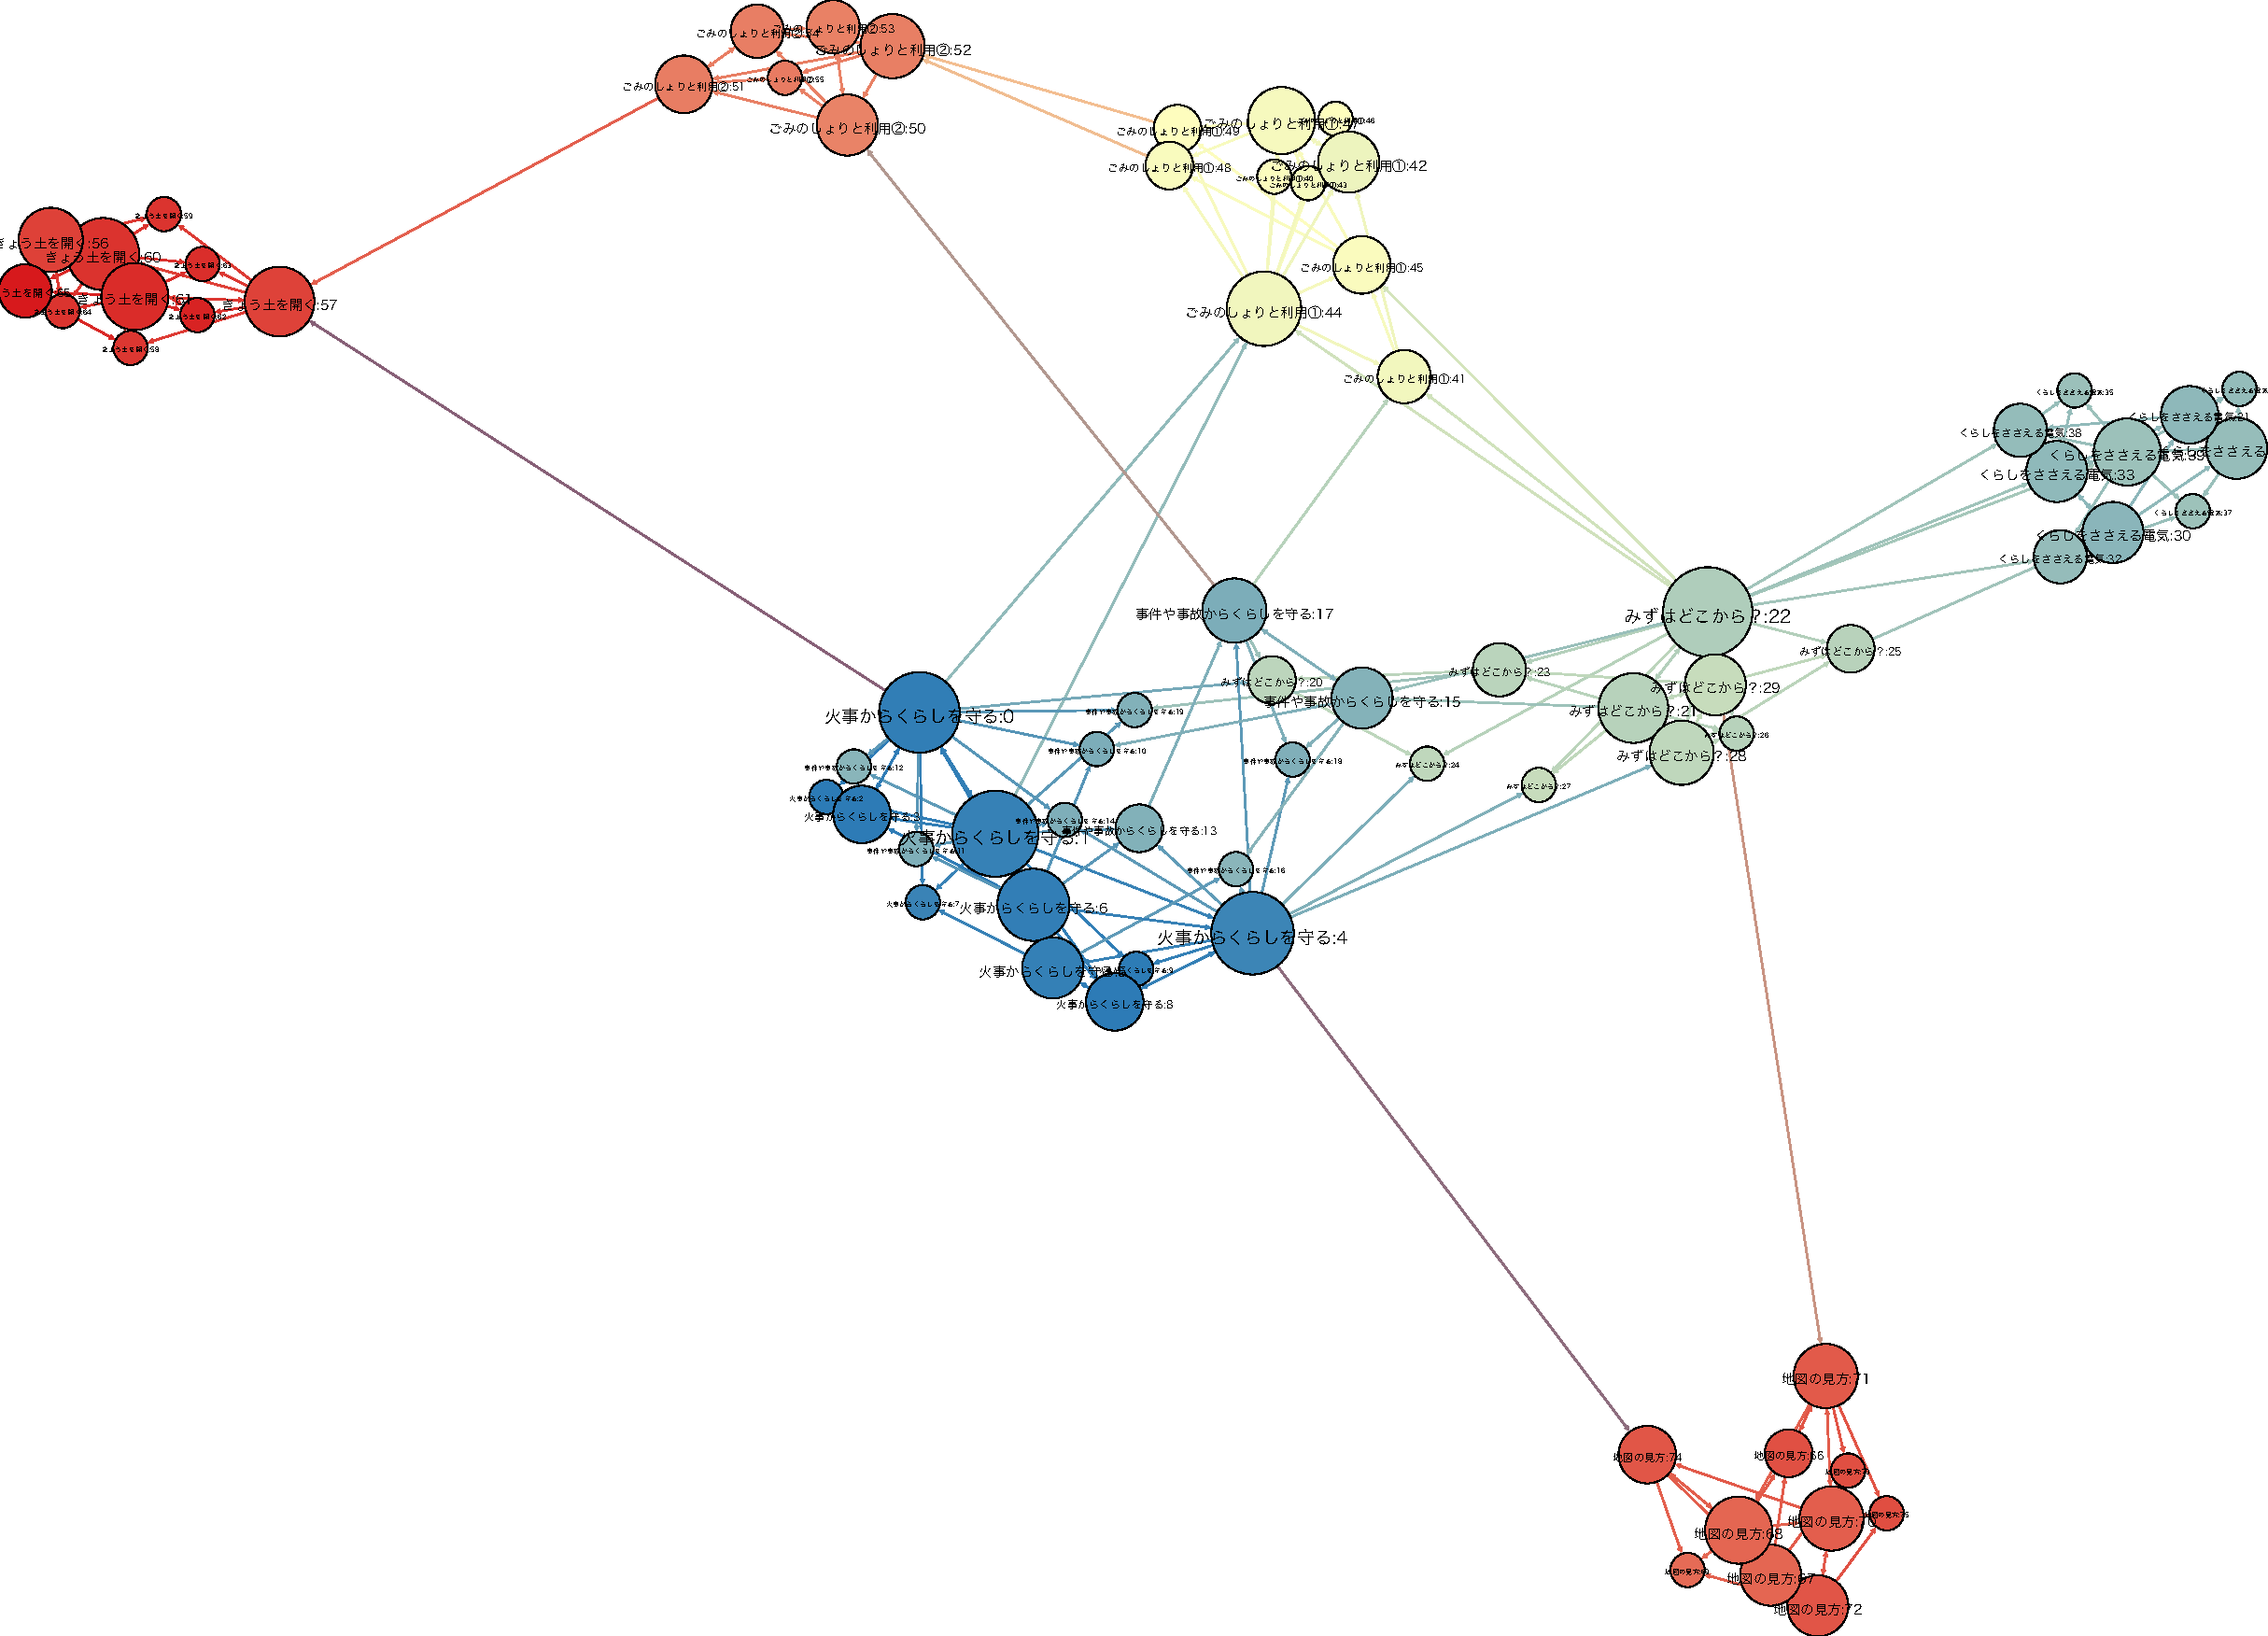
\includegraphics[width=200pt, height=200pt]{./img/net_s4soc.pdf}
			\caption{小学4年社会の問題間関係ネットワーク}
			\label{fig:net_s4soc}
		\endminipage\hfill
		\minipage{0.52\textwidth}
			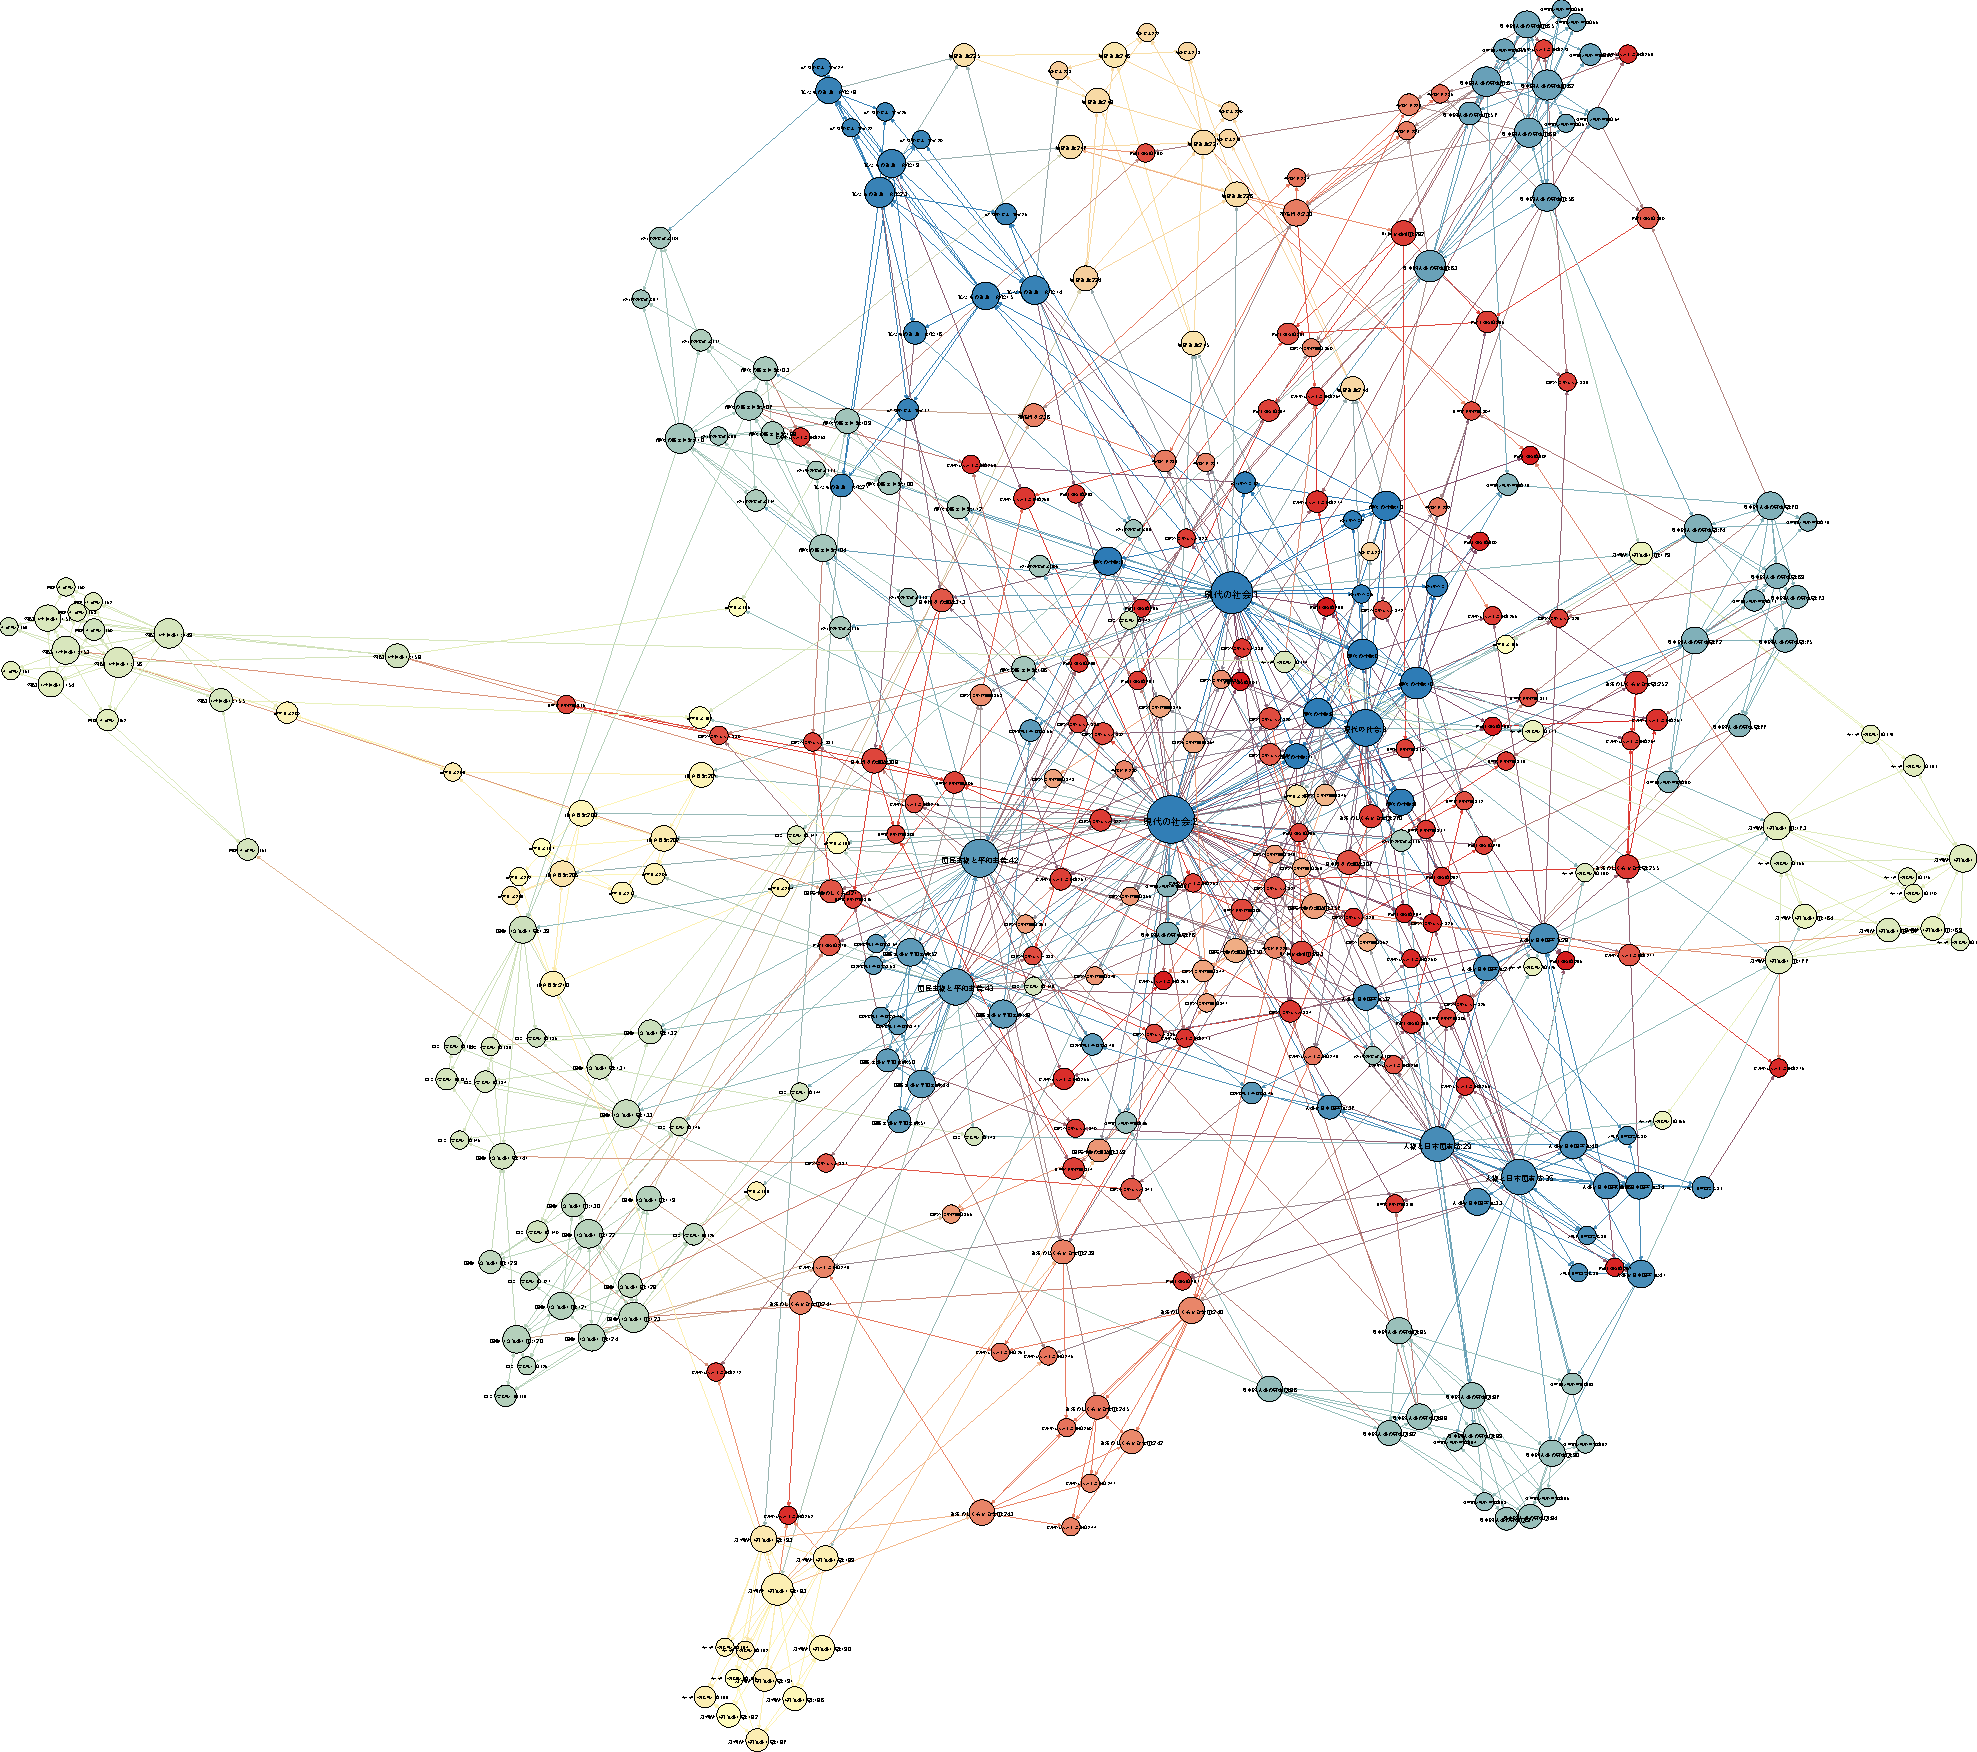
\includegraphics[width=200pt, height=200pt]{./img/net_c_cit.pdf}
			\caption{中学公民の問題間関係ネットワーク}
			\label{fig:net_c_cit}
		\endminipage\hfill
	}
	\hspace*{-10pt}\makebox[1.2\textwidth][c]{
		\minipage{0.52\textwidth}
			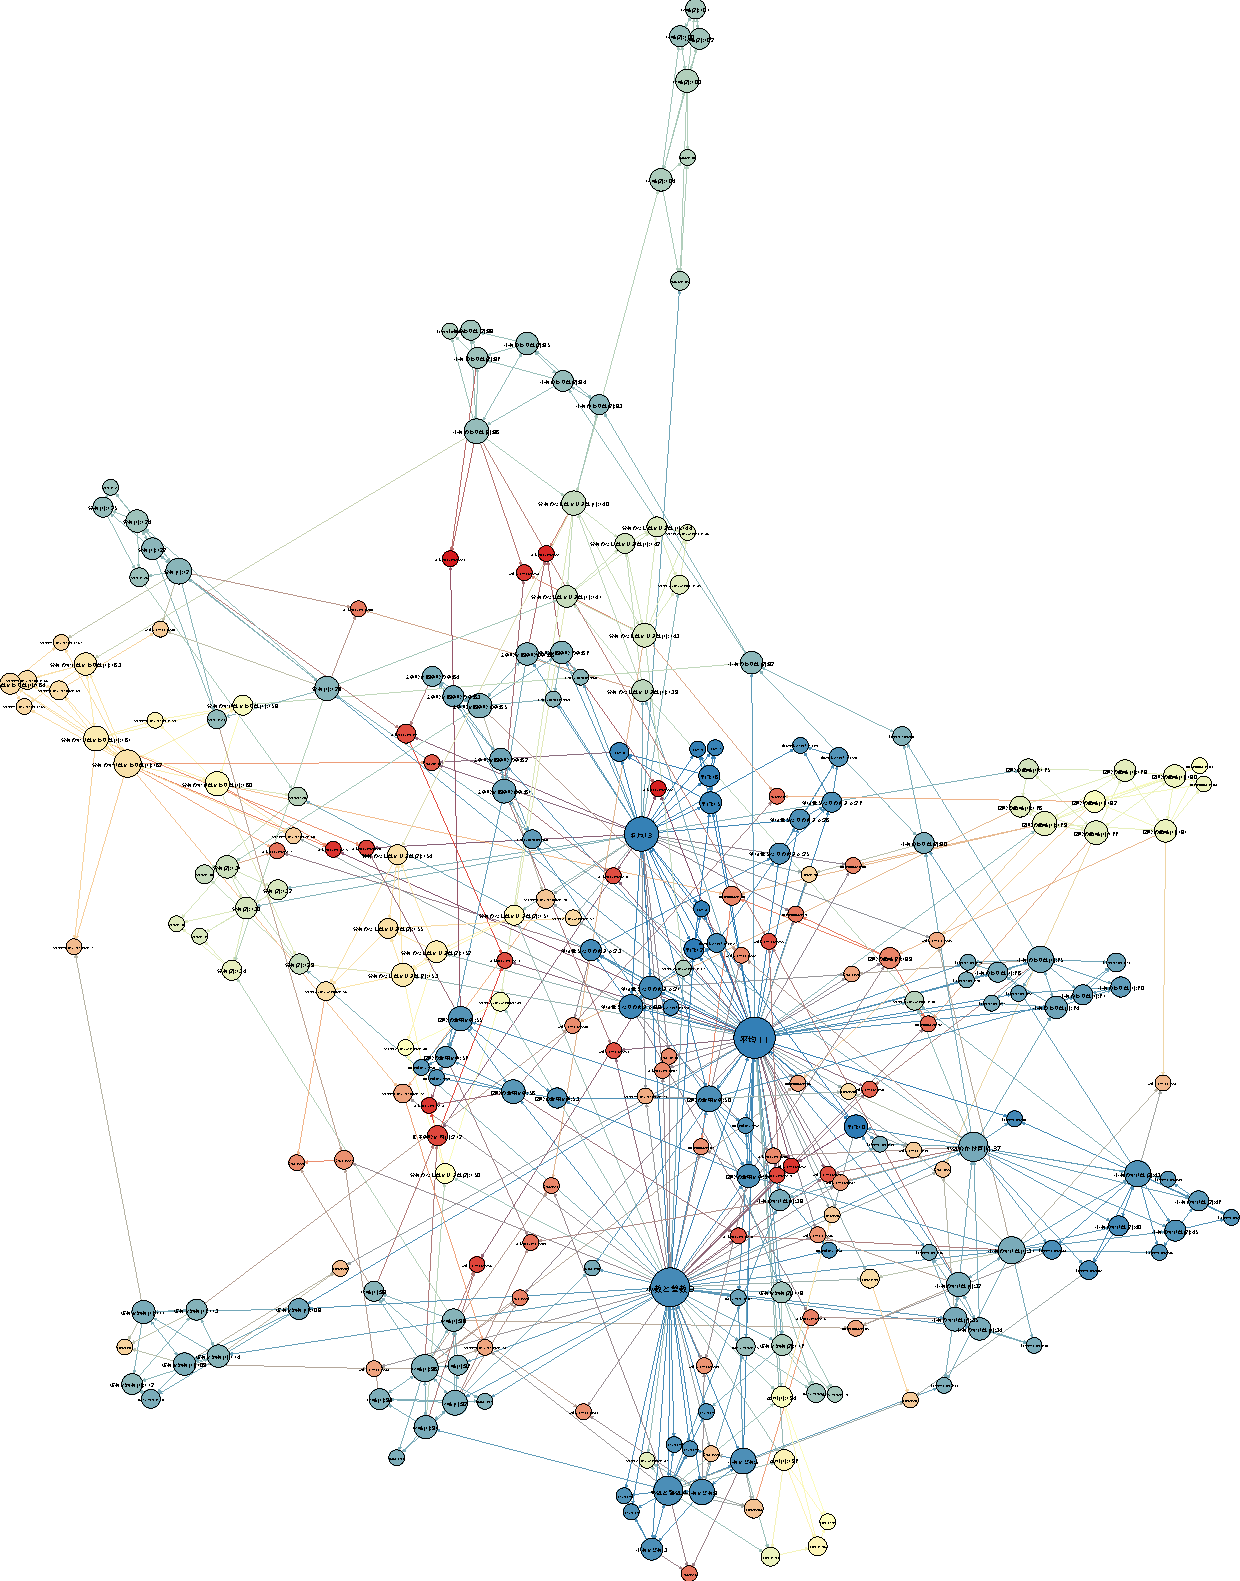
\includegraphics[width=200pt, height=200pt]{./img/net_s5mat.pdf}
			\caption{小学5年算数の問題間関係ネットワーク}
			\label{fig:net_s5_mat}
		\endminipage\hfill
		\minipage{0.52\textwidth}
			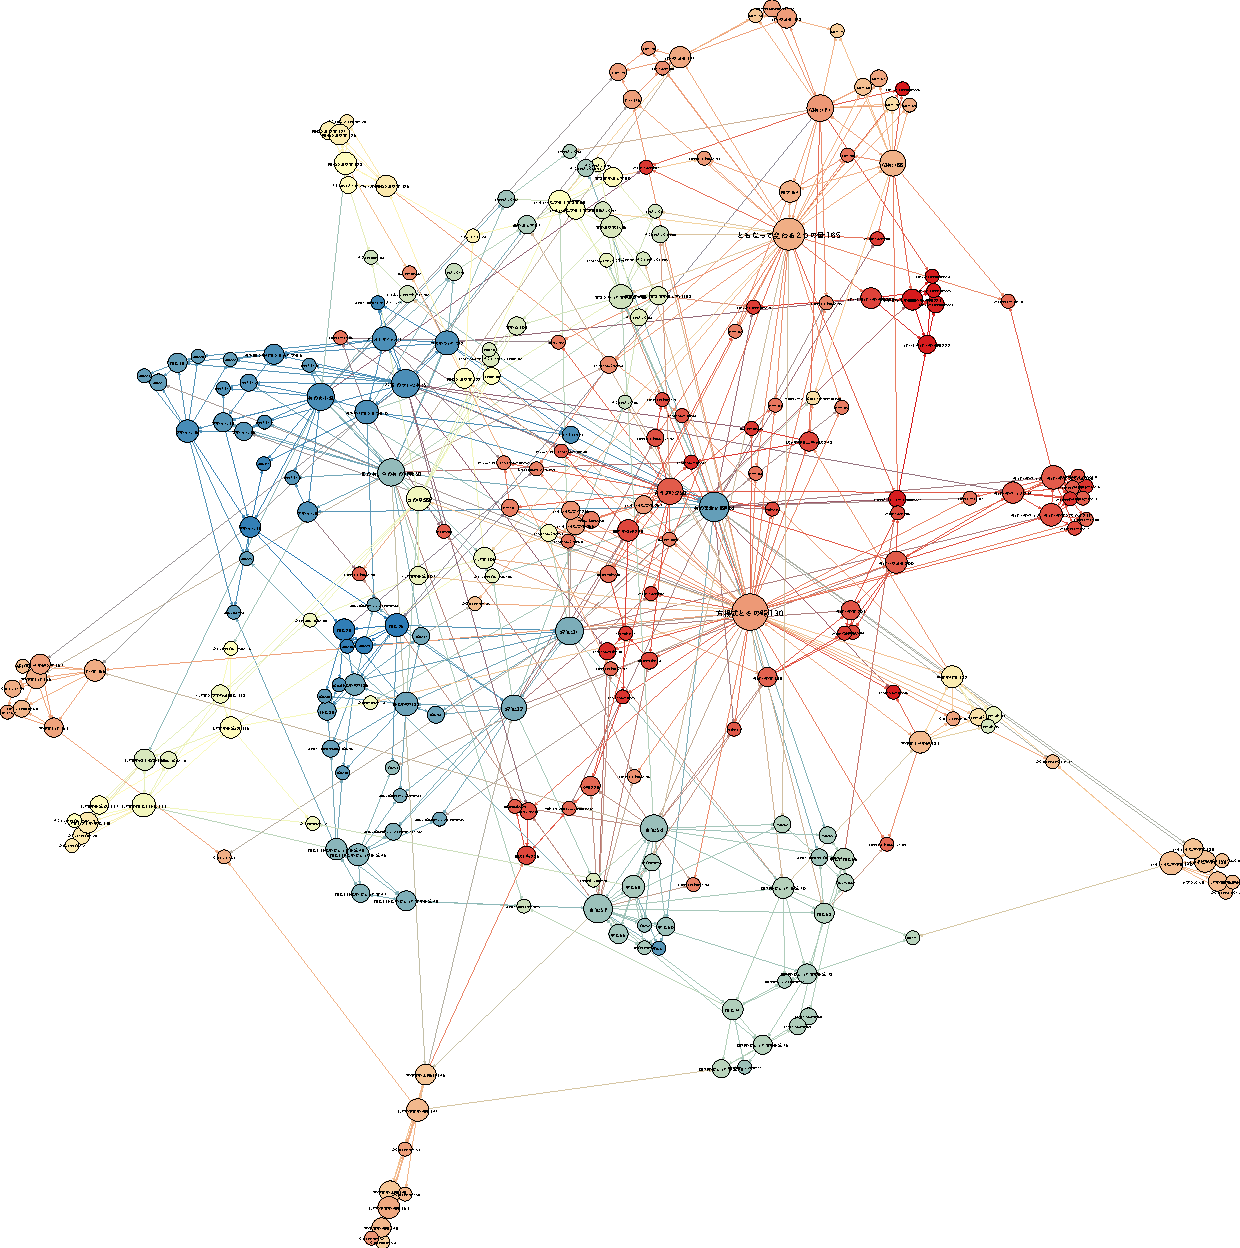
\includegraphics[width=200pt, height=200pt]{./img/net_c1mat.pdf}
			\caption{中学1年数学の問題間関係ネットワーク}
			\label{fig:net_c1mat}
		\endminipage\hfill
	}
\end{center}
\end{figure}

